\section{Clustered Adaptive Kriging - à retirer}\label{sec:CAK}

The filter is obtained by composing three ideas, each answering a limitation left open by the previous one. \Cref{sec:kriging_PF} substitutes a kriged model for the unknown observation function, \cref{sec:AK_PF} restricts that regression to the training data the particle cloud actually needs, and \cref{sec:CAK_PF} splits the cloud when it ceases to be unimodal. Each component is evaluated as soon as it is introduced, so that its own contribution remains visible.

{les résultats numériques sont répartis dans les trois sous-sections plutôt que regroupés. Conséquence à assumer -- le scénario de recalage de terrain est décrit dans la \cref{sec:kriging_PF} et resservira à la \cref{sec:AK_PF}, le scénario magnétique n'apparaît qu'à la \cref{sec:CAK_PF}. Justifier ce second scénario au moment où il arrive plutôt que de le subir : l'anomalie magnétique est nettement moins stationnaire que le relief, c'est donc sur elle que la clusterisation se juge.}

{métriques communes aux trois sous-sections, à poser une fois -- RMSE, ARMSE, taux de convergence par critère de Mahalanobis, temps de calcul par pas. Les deux articles n'emploient pas les mêmes conventions (l'un moyenne sur les runs convergents, l'autre sur tous), il faut trancher et refaire passer les chiffres correspondants.}

\section{Adaptive Kriging Particle Filter}\label{sec:AK_PF}

Assume a navigation scenario similar to that of \cref{sec:Bayesian_estimation}:
\begin{equation}
	\left\{\begin{aligned}
	x_k&=f_k(x_{k-1},w_k)\\
	z_k&=h_k(x_k,n_k)
	\end{aligned}\right.
\end{equation}
with the exception that $h_k$ is unknown, and the observation noise is additive for the sake of simplicity. Since the likelihood density cannot be evaluated without an observation model, Bayesian data fusion is no longer applicable, and we may only rely on inertial navigation to estimate the state $x_k$.

The goal of this section is to ... \textbf{TODO: à compléter}

\subsection{Kriging the Observation Model}

In our scenarios, the observation function describes the measurment of a physical field by an embedded sensor reads at each time step, and which does not change over the course of the mission. Furthermore, we assume that the environment has been sampled before the mission, whether during a previous reconnaissance mission, or using a known but deteriorated map. This is formally modelled by \cref{th:kriging_navigation_assumptions}.

\begin{assumption}[Observation model]\label{th:kriging_navigation_assumptions}
	The observation function is a time-invariant GP, and its noise is an additive Gaussian white noise of covariance matrix $R_k\succeq0$:
	\begin{equation}
		z_k=h(x_k)+n_k,\qquad n_k\sim\mathcal{N}(0,R_k)\label{eq:field_observation}
	\end{equation}
	where $m:\mathbb{R}^{d_x}\to\mathbb{R}^{d_z}$ is the potentially unknown mean of the GP, and $k:\mathbb{R}^{d_x}\times\mathbb{R}^{d_x}\to\mathbb{R}^{d_z}$ is its chosen covariance kernel.

	We also have access to $\tilde{N}\in\mathbb{N}^*$ distinct training inputs $\tilde{\mathbf{x}}$ and their noisy observations $\tilde{\mathbf{z}}$, degraded by a noise of covariance $\tilde{R}\succeq0$, in the sense of \cref{sec:kriging}.
\end{assumption}

Using \cref{th:kriging_navigation_assumptions} and the kriging theory presented in \cref{sec:kriging}, the likelihood follows:
\begin{equation}
	z_k|x_k\sim\mathcal{N}\left(\hat{z}(x_k,\tilde{\mathbf{x}},\tilde{\mathbf{z}},m),\hat{R}(x_k,\tilde{\mathbf{x}})\right)\label{eq:kriged_likelihood}
\end{equation}
where $\hat{z}$ denotes either three kriging estimators of \cref{sec:kriging}, and $\hat{R}$ is the corresponding covariance matrix. \textbf{TODO: dire que $m$ est potentiellement inconnu et mettre $;$ pour séparer les arguments optionnels ?} In particular, $\hat{R}$ already carries the observation noise $R_k$, so it must not be added a second time.

\begin{remark}[Time-varying observation function]
	In full generality, the observed physical field could vary over time, and so the underlying GP would need to  include a temporal input. While the kriging theory perfectly works with this additional parameter, it would require the training data to be sampled over time as well as space.
\end{remark}


{\huge\textbf{TODO: reprendre ici}}

\begin{remark}[Training inputs and particles]\label{th:training_inputs_particles}
	Queried at a particle, $\hat{z}_{\mathrm{OK}}\left(x_k^{(i)},\tilde{\mathbf{x}},\tilde{\mathbf{z}}\right)$ predicts the observation the vehicle would make in the state $x_k^{(i)}$. The training inputs $\tilde{\mathbf{x}}$ share that space without being particles, as they are the states at which the field was sampled before the mission, and remain fixed while the particle set is redrawn at every step.
\end{remark}

\begin{remark}[Altimetric observation]\label{th:altimetric_observation}
	A radar altimeter measures the height of the vehicle above the ground, so its observation function is the difference between the vertical position of the state and the terrain elevation, whereas the prior samples describe the terrain alone. Both differ by a quantity that the queried state fixes, so kriging the terrain and subtracting the estimate from the vertical position of the query yields $h$, and \eqref{eq:kriged_likelihood} applies unchanged. Any observation function depending affinely on a sampled field reduces to \eqref{eq:field_observation} in the same way.
\end{remark}

{points de notation restants, à valider ou à corriger avant d'aller plus loin.}
\begin{itemize}
	\item \textbf{le processus est $f$ au \cref{sec:Gaussian_processes} et $h$ ici.} L'identification est faite en une clause plus haut, ce qui paraît suffisant -- renommer le processus du \cref{sec:Gaussian_processes} serait faux, puisqu'il y est un processus gaussien quelconque et non une fonction d'observation. À relire une fois le chapitre écrit, pour vérifier que la clause tient toute seule ;
	\item \textbf{$h$ perd son indice $k$} ici, alors que le \cref{sec:Bayesian_estimation} écrit $h_k$. La justification est donnée (le champ est statique), mais l'entrée « $h_k$ -- Observation function » de la liste des symboles est à passer en « $h,h_k$ » ;
	\item \textbf{le champ est indexé par l'état entier}, vitesses comprises, alors qu'il n'en dépend pas physiquement. Rien n'est faux tant que le noyau reste aveugle aux composantes de vitesse, mais l'apprentissage des hyperparamètres peut y voir des longueurs de corrélation à estimer. À régler d'un mot au moment de décrire les scénarios, en restreignant $\mathcal{U}$ aux positions ;
	\item \textbf{la \cref{th:altimetric_observation} est à replacer} une fois le scénario altimétrique décrit, si elle arrive trop tôt ici. Sa dernière phrase peut sauter, c'est le seul reste du cas affine général ;
	\item \textbf{à ajouter à la liste des symboles} du \cref{sec:adaptive_kriging} -- $\tilde{N}_c$, $\tilde{N}_f$, $e_r$, $e_f$.
\end{itemize}

{la remarque centrale du chapitre, à soigner -- une interpolation déterministe rend un point sans incertitude, ce qui rend le filtre trop confiant et le fait diverger sur une carte bruitée, alors que $\hat{R}_{\mathrm{OK}}$ élargit la vraisemblance là où la carte est mal connue. C'est l'argument qui justifie le processus gaussien plutôt que l'interpolation bilinéaire, et il vaut mieux que l'argument de précision.}

\begin{remark}[What the surrogate likelihood approximates]\label{th:surrogate_approximation}
	At a given time step, nothing is approximated. \Cref{th:simple_kriging_conditional} identifies the kriged law with the conditional law of $z_k$ given the training data, so \eqref{eq:kriged_likelihood} is the likelihood obtained by integrating the unknown $h$ out, and not a surrogate standing in for it. The weight of a particle involves that law at its own state alone, so the correlation between the errors made at two distinct particles never reaches the weight update. This is why only the block diagonal of the kriging covariance is ever formed.

	Across time steps, on the other hand, the same realisation of $h$ produces every observation of the mission. Given the trajectory, the joint law of $\mathbf{z}_{1:k}$ is Gaussian with the posterior cross-covariances of the field off its diagonal, and is therefore not the product of the marginals \eqref{eq:kriged_likelihood} that the recursion multiplies. Nothing is approximated in the kriging itself, which remains the exact conditional law of $z_k$ given $\tilde{\mathbf{z}}$. What is approximated is the factorisation, since $(x_k)_{k\geq0}$ alone is no longer a sufficient state once every observation is a reading of one and the same unknown field, and \cref{th:observation_independence} fails. Successive observations over a poorly reconstructed area then reinforce one another instead of averaging out, which biases the estimate and leaves the filter more confident than it should be. An exact treatment would condition the model on the observations already collected, hence on the states at which they were acquired, which are precisely the quantities being estimated.

	The neglected quantity is thus the same in both cases, namely the off-diagonal blocks of the kriging covariance. They stay idle between two particles held at the same time step, and do not between two states visited at different ones.

	Inflating the observation noise is the usual guard against this over-counting. It corrects nothing, since $\hat{R}$ already carries the right uncertainty for a single step, but it keeps repeated readings of the same reconstruction error from shrinking the posterior covariance as fast as independent ones would. Discarding observations at the rate at which the field decorrelates has the same effect. Neither restores accuracy, as a reconstruction bias displaces the likelihood peak whatever its width.
\end{remark}

\textbf{TODO: à décider, la remarque ci-dessus s'arrête volontairement au constat.}
\begin{itemize}
	\item \textbf{chiffrer le facteur d'inflation} plutôt que de le laisser qualitatif. Le nombre de pas consécutifs passés à l'intérieur d'une longueur de corrélation du champ vaut $l/(v\Delta_t)$, et c'est l'ordre de grandeur du sur-comptage. Sur le scénario de FUSION 2024 ($\Delta_t=0,5$ s, une centaine de kilomètres en $300$ s), cela fait environ $150$ m parcourus par pas, donc une dizaine de mesures corrélées pour une longueur de corrélation kilométrique -- à recalculer proprement, mais l'ordre de grandeur n'est pas négligeable ;
	\item \textbf{dire ou non que les filtres testés compensent déjà}, sans l'avoir cherché. Le $Q_k$ de FUSION 2024 a été choisi large pour que les particules continuent d'explorer, et la régularisation du RPF réinjecte de la dispersion après chaque rééchantillonnage. Les deux vont contre la surconfiance décrite ici. C'est honnête à écrire, mais cela revient à dire qu'un réglage empirique masque un défaut de modèle, donc à voir si tu veux l'assumer ;
	\item \textbf{la correction propre, à trancher} -- modéliser l'erreur de reconstruction comme un biais d'observation estimé plutôt que la subir. En reprenant la notation $b_k^{(o)}$ du \cref{sec:analytical_estimation}, où elle désigne un biais d'observation connu, l'observation s'écrit $z_k=\hat{z}(x_k,\tilde{\mathbf{x}},\tilde{\mathbf{z}},m)+b_k^{(o)}+n_k$, et le biais suit un processus de Gauss-Markov d'ordre $1$ le long de la trajectoire, $b_k^{(o)}=e^{-\Delta_t/\tau}\:b_{k-1}^{(o)}+\varepsilon_k$ avec $\varepsilon_k\sim\mathcal{N}\left(0,\sigma^2\left(1-e^{-2\Delta_t/\tau}\right)\right)$. Points à développer si l'option est retenue :
	\begin{itemize}
		\item \textbf{pourquoi Gauss-Markov} -- en temps discret, l'autorégressif d'ordre $1$ est le seul processus gaussien stationnaire et markovien. C'est donc le modèle le plus simple qui rende la corrélation sans obliger à porter l'historique dans l'état, et son autocorrélation est exponentielle, de temps caractéristique $\tau$ ;
		\item \textbf{ses paramètres se lisent sur le GP} et ne sont pas libres. La variance stationnaire $\sigma^2$ vaut $\hat{R}-R_k$, et $\tau$ est le temps mis pour parcourir une longueur de corrélation de l'erreur de reconstruction. Or cette longueur est exactement ce que décrivent les blocs hors-diagonaux de $\hat{R}_{\mathrm{SK}}(\mathbf{x},\tilde{\mathbf{x}})$ du \cref{sec:kriging} -- l'augmentation d'état est donc la façon d'exploiter leur contenu en n'en retenant qu'un scalaire, sans jamais former la matrice ;
		\item \textbf{le surcoût est presque nul en filtrage particulaire} -- conditionnellement à la trajectoire d'une particule, $\hat{z}(x_k)$ est un nombre connu et le biais est linéaire-gaussien. C'est la structure exacte du filtre marginalisé du \cref{sec:particle_filtering}, donc chaque particule porte un petit filtre de Kalman sur son biais, sans augmenter la dimension explorée par le nuage ;
		\item \textbf{ce n'est pas qu'une heuristique} -- un GP de noyau de Matérn à $\nu$ demi-entier, au sens de la \cref{th:Matérn_properties}, restreint à une droite admet une représentation d'état linéaire exacte d'ordre $\nu+1/2$, qui se réduit à un Gauss-Markov d'ordre $1$ pour $\nu=1/2$ \cite{bib:Solin-master}. Sur une trajectoire rectiligne, celle des simulations de FUSION 2024, l'augmentation d'état n'est donc pas une approximation du modèle mais sa réécriture exacte. \textbf{La référence canonique de cette correspondance Matérn/EDS manque à \texttt{biblio.bib}} et serait à ajouter si le point est développé ;
		\item \textbf{ce que le modèle ne rend pas} -- l'erreur est indexée par la position et non par le temps. Sur un passage unique la correspondance est bonne, mais un croisement de trajectoire devrait redonner la même erreur, ce qu'un processus temporel a oublié. C'est une fermeture de boucle, et c'est précisément ce qu'une estimation conjointe du champ traiterait. De même, $\tau$ dépend de la vitesse, ce qui se corrige en indexant le processus par la distance parcourue plutôt que par le temps.
	\end{itemize}
\end{itemize}

{schéma d'ensemble de la chaîne (centrale inertielle, altimètre, sélection des données, régression, filtre), repris de la figure~1 du poster \cite{bib:data-selection}. C'est la seule figure du chapitre qui montre l'architecture complète, elle a sa place ici.}

{scénario de recalage de terrain -- modèle d'observation altimétrique, état à six composantes, mouvement rectiligne uniforme (\texttt{Schéma de la corrélation de terrain.pdf}), carte et relief survolé (\texttt{Carte altimétrique FUSION 2024.pdf}, \texttt{Élévation de terrain FUSION 2024.pdf}), en soulignant l'ambiguïté du terrain plat entre les deux cuvettes.}

{campagne Monte-Carlo à trois termes -- filtre sur carte complète non bruitée (cas idéal), filtre sur carte bilinéaire dégradée, filtre krigé (\texttt{RMSEs FUSION 2024.png}, \texttt{Trajectoire FUSION 2024.png}).}
\begin{itemize}
	\item taux de convergence et RMSE en fonction du nombre de points d'apprentissage, jusqu'au décrochage. Le résultat marquant est que le filtre krigé converge avec environ huit fois moins de points que l'interpolation bilinéaire n'en demande pour atteindre la moitié du même taux ;
	\item effet du bruit de carte $\tilde{R}$ à densité fixée, et effet d'un échantillonnage irrégulier plutôt qu'en maillage régulier ;
	\item l'analyse à conserver -- la RMSE chute au passage des reliefs informatifs et remonte sur le terrain plat, et le krigeage extrait plus d'information de ces reliefs que l'interpolation bilinéaire parce qu'il lisse le bruit de carte au lieu de le propager.
\end{itemize}

{vérifier de quel document il s'agit -- « poster 1A » ne correspond peut-être pas à \cite{bib:data-selection}, qui est daté de 2025 et porte sur les méthodes de sélection, donc plutôt sur la \cref{sec:AK_PF}. S'il s'agit d'un poster de première année distinct, il lui faut sa propre entrée dans \texttt{biblio.bib}.}

\section{Adaptive Kriging Particle Filter - à incorporer dans la section d'avant}\label{sec:AK_PF1}

Two independent difficulties rule out using the whole training set at every step. One is a matter of cost, the other of modelling.

{développer les deux, dans cet ordre, en insistant sur leur indépendance -- même à coût nul, l'ajustement global resterait mauvais.}
\begin{itemize}
	\item \textbf{Coût.} Inversion en $\mathcal{O}(\tilde{N}^3)$ à chaque pas, plus $\mathcal{O}(\tilde{N}^2)$ par particule, à quoi s'ajoute la descente de gradient de l'apprentissage des hyperparamètres. Chiffrer sur la carte du scénario de la \cref{sec:kriging_PF} pour rendre l'ordre de grandeur concret ;
	\item \textbf{Non-stationnarité.} Un relief n'a pas la même longueur de corrélation partout. Estimer un unique $\theta$ par vraisemblance marginale sur l'ensemble de la carte produit un compromis qui ne décrit correctement aucune région, et le krigeage qui en découle est mal calibré -- trop lisse là où le champ varie vite, trop nerveux ailleurs. Rapprocher des noyaux non stationnaires \cite{bib:non-stationary-GP} et des approximations locales de GP \cite{bib:local-GP}, en précisant le choix fait ici, qui est de garder un noyau stationnaire et de le ré-ajuster localement plutôt que de complexifier le noyau.
\end{itemize}

{méthodes de sélection des données, d'après le poster \cite{bib:data-selection} qui en compare trois, avec \cref{fig:data_selection} en support. Renvoyer à la \cref{sec:subsampling_error} pour le chiffrage de l'erreur, et se contenter ici de l'argument qualitatif -- la covariance décroît avec la distance, donc un point d'apprentissage éloigné de toutes les particules ne pèse presque rien.}
\begin{itemize}
	\item décimation aléatoire ou régulière du maillage, indépendante des points de requête ;
	\item plus proches voisins par particule -- le plus informatif, mais une inversion par particule ;
	\item fenêtre globale contenant tout le nuage -- une seule inversion partagée, au prix de données inutiles quand le nuage est étalé.
\end{itemize}

\begin{figure}[!htb]
	\centering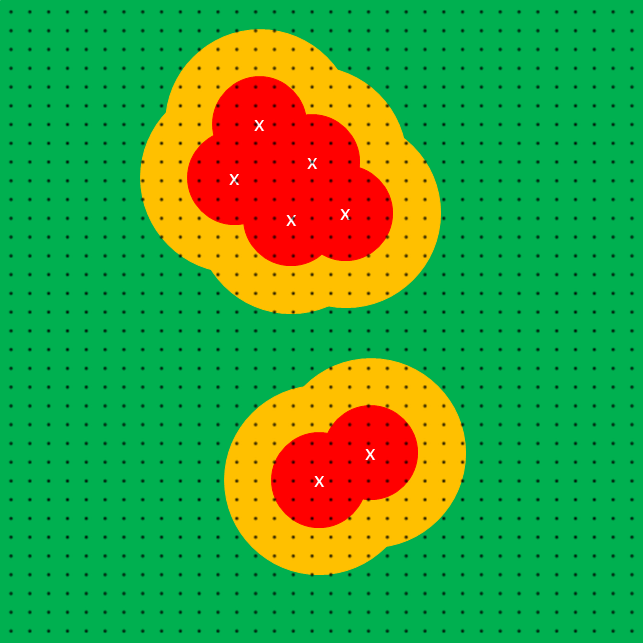
\includegraphics[width=0.6\textwidth]{../../Images/Sélection des données de krigeage.png}
	\caption{Training points retained by three selection strategies. \textbf{(légende à réécrire une fois la figure refaite : préciser le code couleur)}}\label{fig:data_selection}
\end{figure}

The retained training points are those lying in a ball centred on the predicted state, whose radius follows the predicted uncertainty:
\begin{equation}
	\mathcal{S}_k\triangleq\left\{i\in[\![1,\tilde{N}]\!]\:\middle|\:\tilde{x}_i\in\mathcal{B}\left(\hat{x}_{k|k-1},r_k\right)\right\}
\end{equation}
with a radius proportional to the semi-major axis of the $3\sigma$-ellipsoid of $P_{k|k-1}$, enlarged so that most particles are interpolated rather than extrapolated, and dilated further if fewer than $\tilde{N}_{\min}$ points would be retained.

\begin{itemize}
	\item écrire $r_k$ et $\alpha_{\mathrm{sel}}$ proprement, et discuter le choix de $\tilde{N}_{\min}$ ;
	\item projeter sur les composantes de position, le rayon n'ayant de sens que sur $\mathcal{U}$ et pas sur les vitesses -- c'était $\pi_g$ dans FUSION 2024, à renommer ;
	\item \cref{fig:kriging_window} pour le schéma de la fenêtre ;
	\item apprentissage local des hyperparamètres -- appliquer \cref{th:GP_MLE} aux seules données retenues, avec initialisation à chaud par $\theta_{k-1}$. C'est le point où les deux difficultés ci-dessus se résolvent d'un même geste, et où le sur-ajustement sur une fenêtre presque vide motive $\tilde{N}_{\min}$ ;
	\item complexité de l'ensemble, à comparer à celle du krigeage complet.
\end{itemize}

\begin{figure}[!htb]
	\centering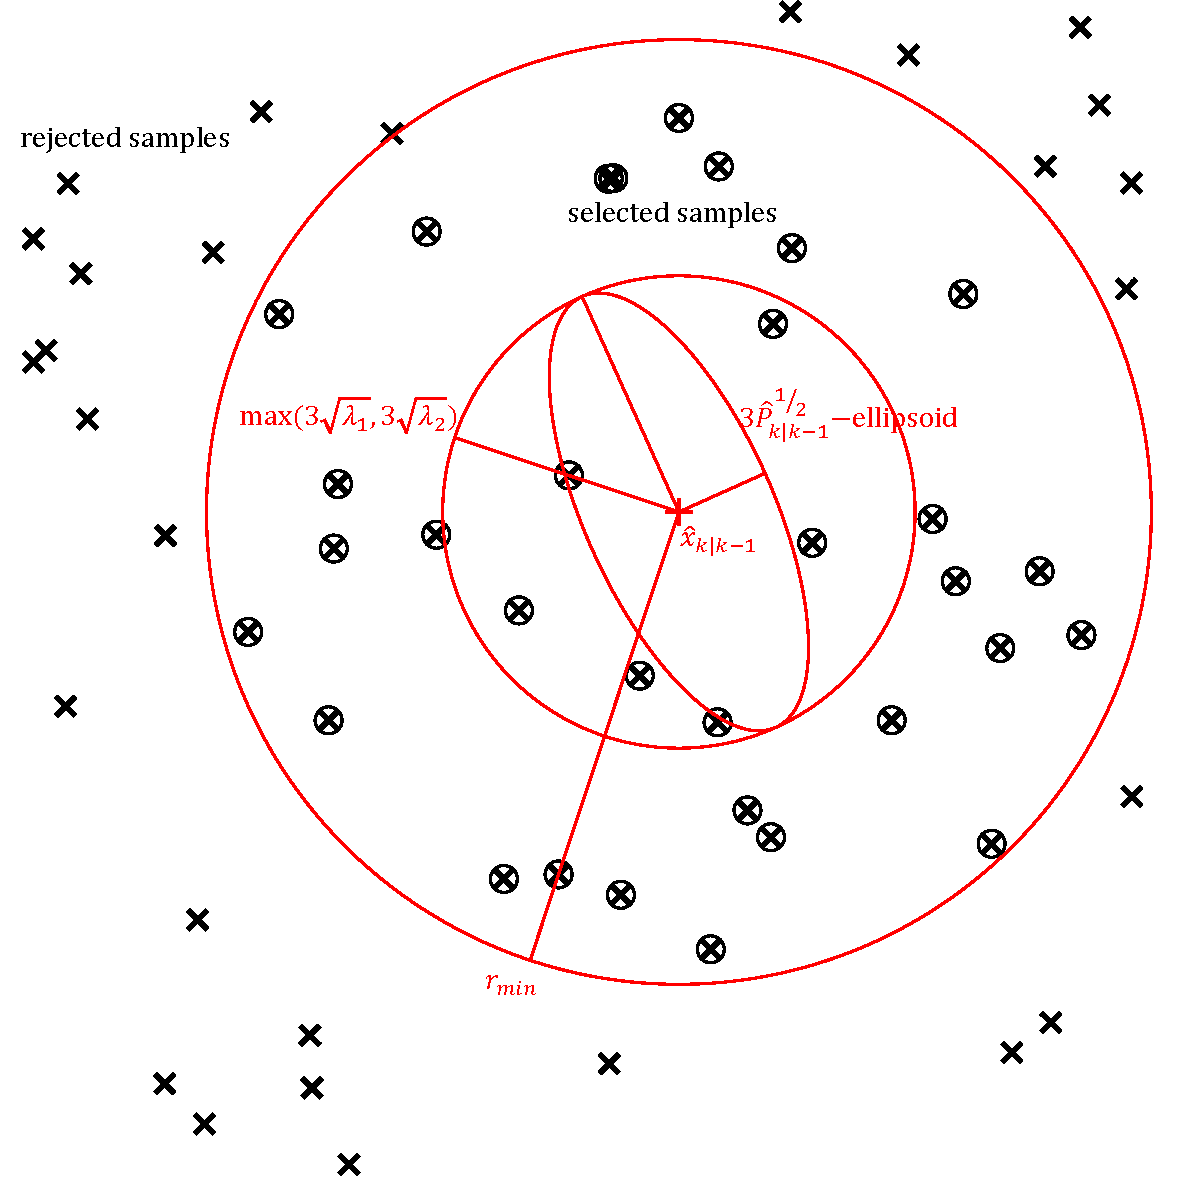
\includegraphics[width=0.6\textwidth]{../../Images/Fenêtrage du krigeage adaptatif.pdf}
	\caption{Adaptive kriging window, obtained as the circumscribed circle of the $3\sigma$-ellipsoid of the predicted state dilated by $\alpha_{\mathrm{sel}}$}\label{fig:kriging_window}
\end{figure}

{algorithme AK-PF, greffé sur le filtre générique du \cref{sec:particle_filtering}, avec les étapes sélection $\to$ hyperparamètres $\to$ krigeage insérées avant la mise à jour des poids. Pas d'étape d'estimation dans la boîte. Remarque sur le filtre support -- FUSION 2024 utilise le RPF, la méthode est indifférente au filtre sous-jacent et le choix se discute par régime de bruit, comme au \cref{sec:particle_filtering}. Figure candidate : \texttt{Exemple RPF avec krigeage.png}.}

{sur le même scénario que la \cref{sec:kriging_PF}, de sorte que seules les briques ajoutées expliquent l'écart.}
\begin{itemize}
	\item comparaison des trois méthodes de sélection à l'intérieur du filtre, à budget de calcul égal, et pas seulement sur le krigeage seul ;
	\item sensibilité à $\alpha_{\mathrm{sel}}$ et à $\tilde{N}_{\min}$, avec la dégradation attendue aux deux extrêmes -- fenêtre trop étroite qui extrapole, fenêtre trop large qui retombe sur le krigeage complet ;
	\item apport propre de l'apprentissage des hyperparamètres, en gelant $\theta$ à sa valeur initiale. C'est la seule expérience qui sépare l'effet « moins de données » de l'effet « bon noyau local » ;
	\item temps de calcul par pas pour chaque réglage, en regard de la RMSE -- c'est l'argument principal du poster, la performance temps réel s'améliore sans perte de précision ni de taux de convergence.
\end{itemize}

\section{Clustered Adaptive Kriging Particle Filter}\label{sec:CAK_PF}

A single window is only economical while the particles stay together. Under a high initial uncertainty or an ambiguous field, the posterior becomes multimodal and the cloud splits, at which point a ball containing every particle also covers the empty space between the modes.

{développer le constat, en gardant les trois arguments distincts.}
\begin{itemize}
	\item la fenêtre est dimensionnée par $P_{k|k-1}$, qui mesure l'étalement global et non la taille des modes, donc son rayon croît avec la séparation entre modes et non avec l'incertitude réelle de chacun ;
	\item les données ramassées entre les modes sont payées à l'inversion sans servir aucune particule. Le nombre de données d'entraînement effectivement utilisées, et donc le temps de calcul, est ainsi piloté par la multimodalité bien plus que par la précision recherchée ;
	\item des modes séparés de plusieurs dizaines de kilomètres n'ont aucune raison de partager une longueur de corrélation, ce qui ramène le problème de non-stationnarité que la \cref{sec:AK_PF} venait de résoudre.
\end{itemize}

{rappeler que la multimodalité est le régime normal en recalage de terrain et non un cas pathologique -- c'est la raison d'être du filtrage particulaire ici. Citer la thèse d'Achille Murangira \cite{bib:these-Murangira} sur les approches particulaires en recalage inertiel, et éventuellement \cite{bib:these-Dahia,bib:these-Palmier} pour la même lignée à l'ONERA.}

{comparer les familles d'algorithmes de partition avant de justifier le choix, plutôt que de présenter le décalage vers la moyenne seul.}
\begin{itemize}
	\item méthodes à nombre de classes imposé, $k$-moyennes ou mélange gaussien par espérance-maximisation -- inutilisables telles quelles, puisque le nombre de modes varie le long de la trajectoire et n'est pas observable ;
	\item méthodes par densité, DBSCAN et apparentées -- pas de nombre de classes à fournir, mais un rayon de voisinage et un effectif minimal qui jouent le même rôle de réglage caché ;
	\item décalage vers la moyenne \cite{bib:mean-shift,bib:mean-shift-clustering} -- non paramétrique, le nombre de classes est un résultat et non une entrée, au prix d'une largeur de bande. C'est le choix retenu, et il se raccorde naturellement à l'estimation par noyau du \cref{sec:particle_filtering}, puisqu'il s'agit de la même densité lissée, dont on cherche ici les maxima locaux au lieu d'y rééchantillonner.
\end{itemize}

{définir la suite de décalage et les classes comme classes d'équivalence de la relation « converger vers le même maximum », donner le coût $\mathcal{O}(TN^2)$ et le nombre d'itérations observé en pratique, et illustrer par la \cref{fig:clustering}.}

\begin{figure}[!htb]
	\centering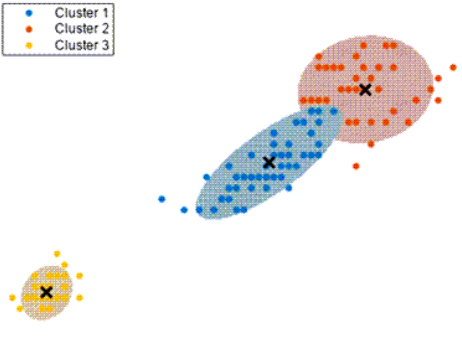
\includegraphics[width=0.6\textwidth]{../../Images/Exemple de clustering.png}
	\caption{Partition of a multimodal particle cloud by mean-shift, with the $1\sigma$-ellipsoid and the mode of each cluster}\label{fig:clustering}
\end{figure}

{fenêtrage multimodal -- transposer la \cref{sec:AK_PF} à chaque classe (poids renormalisés, moyenne et covariance prédites par classe, fenêtre et hyperparamètres propres), ce qui revient à un modèle stationnaire par morceaux. Insister sur le point d'EUSIPCO 2025 : les fenêtres sont indépendantes, chaque classe ignore les données sélectionnées par les autres, et les inversions sont de taille $\tilde{N}_{\mathcal{S}_k^{(l)}}$ et non de leur somme. Remarque sur la discontinuité du modèle aux frontières de classes, sans conséquence tant qu'aucune particule ne s'y trouve.}

{algorithme CAK-PF -- pré-propagation, clusterisation, boucle sur les classes (sélection, hyperparamètres, krigeage, pré-correction), rééchantillonnage des indices parents, propagation, correction. Point à ne pas perdre : avec l'APF, les particules auxiliaires et les particules propagées partagent classes et hyperparamètres, ce qui évite de refaire la clusterisation et l'apprentissage entre les deux corrections. Le justifier par le fait que $\mu_k^{(i)}$ est construite pour représenter $x_k^{(i)}$.}

{complexité algorithmique par étape (décalage vers la moyenne, sélection, apprentissage, krigeage), puis comparaison des trois régimes -- krigeage complet, adaptatif, adaptatif clusterisé. Reprendre le calcul d'EUSIPCO 2025 en le rendant lisible, et surtout en explicitant que l'histogramme cumule les données de toutes les classes alors que les inversions, elles, sont séparées.}

\subsubsection*{Numerical results}

{scénario de navigation par anomalie magnétique \cite{bib:magnetic-navigation} -- état à quatre composantes, carte du Mexique (\texttt{Carte magnétométrique EUSIPCO 2025.png}, \texttt{Anomalie magnétique EUSIPCO 2025.pdf}).}
\begin{itemize}
	\item comparaison des quatre filtres d'EUSIPCO 2025 -- carte connue, krigeage complet, adaptatif, adaptatif clusterisé (\texttt{RMSE EUSIPCO 2025.png}). Le krigeage complet décroche hors de la zone où ses hyperparamètres ont été ajustés, ce qui est la démonstration directe de l'argument de non-stationnarité ;
	\item histogramme du nombre de données krigées (\texttt{Histogramme du nombre de données krigées EUSIPCO 2025.png}) -- les médianes des deux méthodes adaptatives sont proches, c'est la queue haute qui les sépare, et elle correspond exactement aux instants multimodaux ;
	\item nombre de classes le long de la trajectoire, à mettre en regard des instants où la version non clusterisée décroche ;
	\item décalage vers la moyenne contre partition à nombre de classes fixé, pour chiffrer ce que coûte de devoir choisir ce nombre, et sensibilité à la largeur de bande ;
	\item temps de calcul par pas et sa dispersion -- l'argument temps réel tient à la régularité du coût autant qu'à sa moyenne ;
	\item trajectoires (\texttt{Trajectoire EUSIPCO 2025 large.png}, \texttt{Trajectoire EUSIPCO 2025 fin.pdf}).
\end{itemize}
